Two lines are parallel if their respective directional vectors are in the same ratio.\\
Let the points be denoted by:
 \begin{align}
     \vec{A}= \myvec{2 \\1}\\
     \vec{B}= \myvec{5 \\4}\\
     \vec{C}=\myvec{4 \\7}\\
      \vec{D}=\myvec{1 \\4 }
 \end{align}
 The directional vector of $\vec{AB}$ is
\begin{align}
\myvec{2-5\\1-4}=\myvec{-3 \\-3}
\end{align}
The directional vector of $\vec{BC}$ is
\begin{align}
\myvec{5-4\\4-7}=\myvec{1 \\-3}
\end{align}
The directional vector of $\vec{CD}$ is
\begin{align}
\myvec{4-1\\7-4}=\myvec{3 \\3}
\end{align}
The directional vector of $\vec{AD}$ is
\begin{align}
\myvec{2-1\\1-4}=\myvec{1 \\-3}
\end{align}
The directional vector of $\vec{AC}$ is
\begin{align}
\myvec{2-4\\1-7}=\myvec{-2 \\-6}
\end{align}
Since the directional vectors of $\vec{AB}$ and $\vec{CD}$ are in the same ratio, so $\vec{AB}$ and $\vec{CD}$ are parallel and also opposite to each other.\\
Similarly, the directional vectors of $\vec{BC}$ and $\vec{AD}$ are in the same ratio,hence $\vec{BC}$ and $\vec{AD}$ are parallel and opposite.\\ 
Since the two pairs of opposite sides are parallel, the given points are the vertices of the parallelogram.\\

Moreover the sum of the directional vectors of $\vec{AB}$ and $\vec{BC}$ \\
  
\myvec{-3\\-3}+\myvec{1 \\-3}= \myvec{-3+1 \\-3-3}=\myvec{-2 \\-6}\\

Thus $\vec{AB}$ $+$ $\vec{BC}$= $\vec{AC}$, which satisfy
parallelogram law of vector addition i.e vector
sum of two adjacent side of a parallelogram is the
diagonal vector of the parallelogram.  See Fig.     \ref{eq:solutions/1/1/3/myfig:1}

\begin{figure}[!]
 \begin{center}
  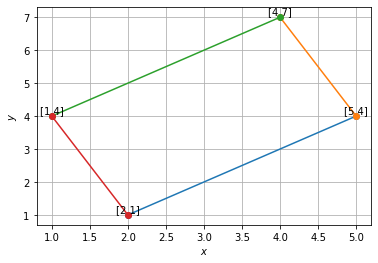
\includegraphics[width=\columnwidth]{solutions/1/1/3/assignment2_fig.png}
    \caption{This is the 2D diagram of the parallelogram with the given vertices}
    \label{eq:solutions/1/1/3/myfig:1}
    \end{center}
\end{figure}
